\section{簡介}
由於第\ref{ch4}章,專注式機制對於系統表現有蠻大的幫助。且第\ref{ch5}章中,非監督式學習的語音詞向量,也有小幅的贏過動態時間規劃,若能夠將部分有標注的資料去微調模型,說不定能有更大的進步。所以在此章中,想將第\ref{ch5}章的語音詞向量跟第\ref{ch4}的專注式機制合併,變成半監督式學習法(Semi-Supervised),使用部分標記資料跟部分非標記資料來訓練,希望進而相輔相成,使其效能能夠更進步。
\section{模型架構}
\subsection{模型簡介}
圖\ref{ch6_model}為本章的模型架構圖,跟第\ref{ch4}章提出的模型幾乎相同。相同地,語音文件跟語音查詢詞都會先從音訊檔案中抽取聲學特徵。接著遞迴類神經網路編碼器將語音查詢詞之聲學特徵轉變成語音查詢詞向量$V_Q$,如圖\ref{ch4_att}(A),而語音文件向量則是採用專注式機制,利用語音查詢詞向量$V_Q$跟每個時間點的語音文件去計算餘弦相似度當作專注式權重,最後依照權重得到語音文件向量$V_D$,如圖\ref{ch4_att}(B)所示。得到$V_Q$跟$V_D$後,丟入分類器產生查詢詞出現在文件的機率。唯一不同的是產生的查詢詞向量跟語音文件向量,必須經過解碼器還原成原本的語音序列。可以將此部分視為一種正規化,希望模型同時能夠分類的精準,同時也能確保產生出的向量表示不會喪失原本語音序列的特徵。

\begin{figure}[h]
\centering
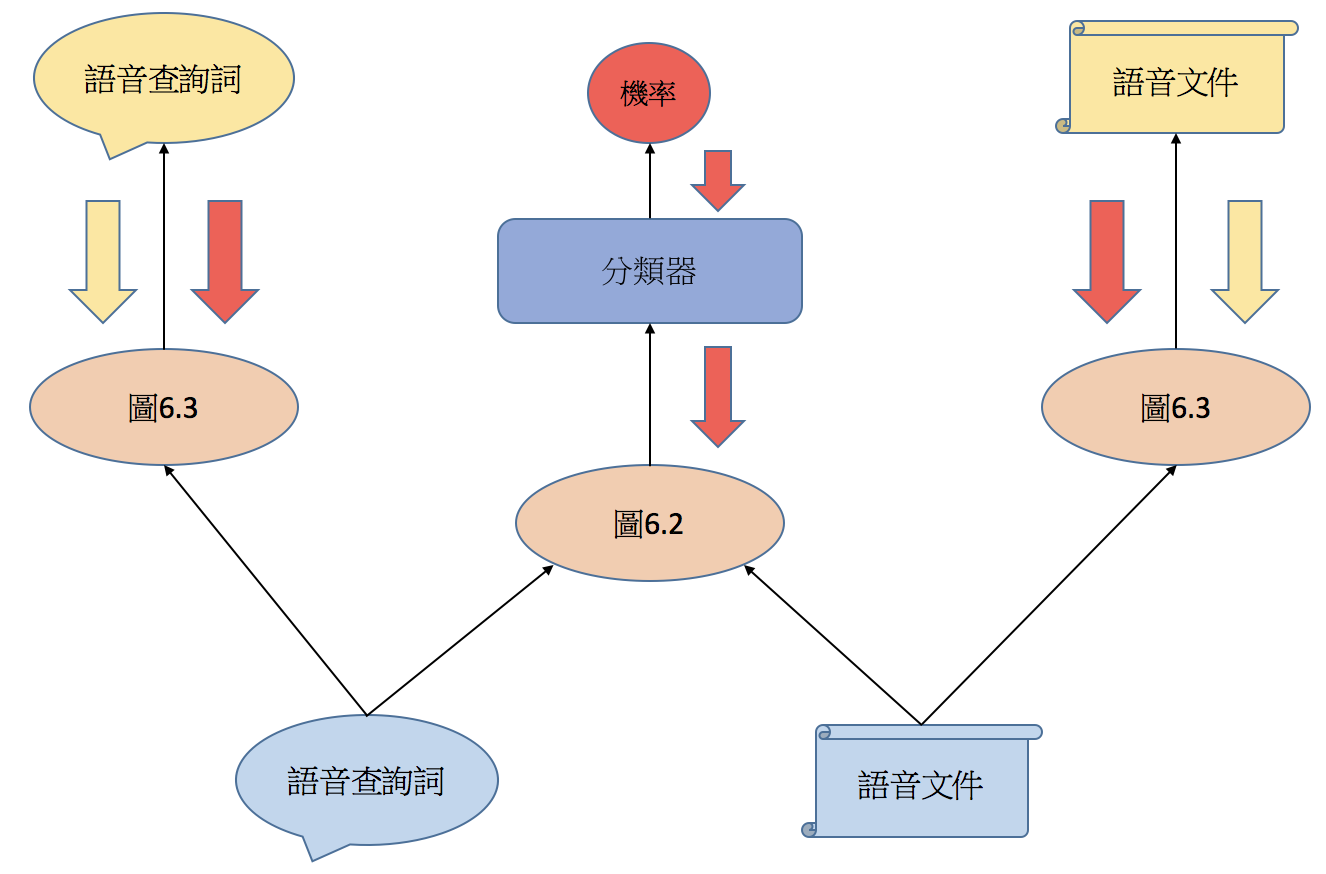
\includegraphics[scale=0.5]{images/ch6_model.png} 
\caption{模型架構圖}
\label{ch6_model}
\end{figure}
\subsection{訓練方式}
此時因模型為多任務學習(Multi-Task
Learning),模型需要同時分類正確,且能夠還原成原本的語音序列。其損失函數會對於其任務有所不同,其一為交叉熵如式\ref{eq:ch5_LCE},為了提高口述詞彙偵測的正確率。
\begin{equation}
\label{eq:ch5_LCE}
L_{CE}(\bold{x} , \bold{y} , \theta) =KL(\bold{y} || f_{\theta}(\bold{x}))= KL( \bold{y} ||\hat{\bold {y}} )  = - \log \hat{y}_{l} 
\end{equation}
其中KL為克雷散度,$\bold{y}$為正確答案,$\hat{\bold{y}}$為模型預測之結果,$\hat{y_l}$為模型給正確標籤的分數。
而另一個損失函數為均方根差\ref{eq:ch5_RMSE},使其編碼向量能夠能夠完整還原最初之語音序列。
\begin{equation}
\label{eq:ch5_RMSE}
L_{rmse} (\bold{x},\bold{y}) = \sum_{i=1}^{T}
RMSE(\bold{x}_i-\bold{y}_i) = \sum_{i=1}^{T} \sum_{j=1}^D \sqrt{(x_{ij}-y_{ij})^2}
\end{equation}
其中RMSE為方均根差,$\bold{x}$為輸入之語音序列,$\bold{y}$為模型還原之語音序列,$\bold{x}_i$為時間點$i$之聲學特徵,$\bold{y}_i$
為時間點$i$之模型還原聲學特徵,T為輸入序列長度,D為聲學特徵向量維度。
\section{實驗與分析}
\begin{itemize}
\item{實驗設定}

	訓練語料為LIBRISPEECH 的英語語料,從train-clean-360
	取出30,000個語音文件當作訓練語料,用來訓練語音詞向量;取出70,000筆查詢詞跟語音文件配對,查詢詞共500個,用來訓練分類器。測試語料跟章節\ref{ch4}的設定相同,分成測試集$1$(查詢詞聲學特徵跟訓練語料相同)、測試集$2$(查詢詞聲學特徵跟測試集不同)、測試集$3$(查詢詞未出現在訓練語料)。
	
	在訓練的時候,會先訓練語音詞向量的部分,為監督式學習的部分,如圖\ref{ch6_model}上黃色箭頭的部分。接著才會訓練分類器。而在訓練分類器的同時,也會同時希望能夠還原成初始的語音序列,如圖\ref{ch6_model}上藍色箭頭部分。
\item{基準實驗}

	基準實驗仍為利用動態時間規劃得到的分數,在分別在測試集$1$得到0.6173的平均準確率,測試集$2$得到0.5778的平均準確率,測試集$3$得到0.5668的平均準確率
\end{itemize}
\section{本章總結}

